\usetikzlibrary{calc}
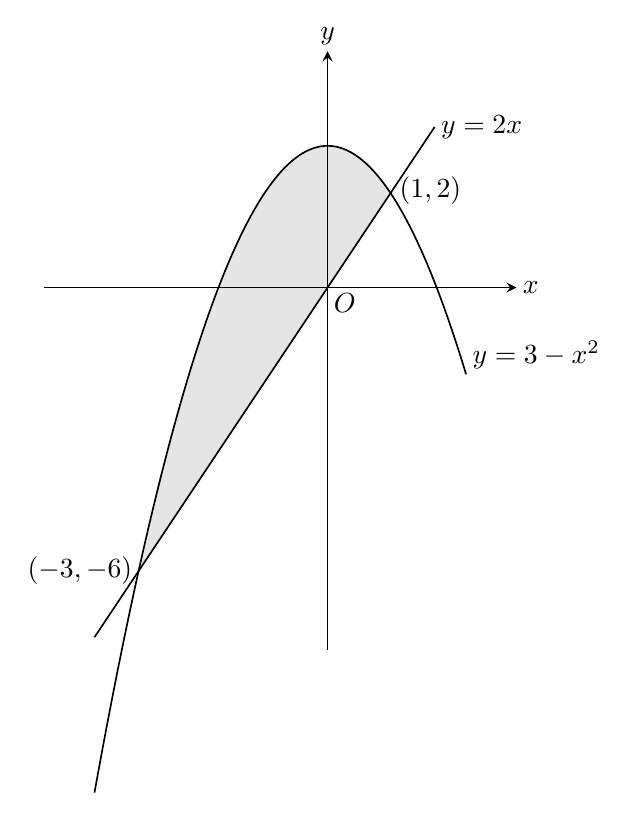
\begin{tikzpicture}[x=1mm,y=1mm,line width=.6pt,>=stealth]
% closed shaded region first, axes and curves on top so strokes stay solid
\fill[gray!20] plot[domain=-3:1,samples=61] ({8*\x},{6*(3-\x*\x)}) -- plot[domain=1:-3,samples=61] ({8*\x},{6*(2*\x)}) -- cycle;
% axes
\draw[->] (-36,0)--(24,0) node[right,inner sep=0pt,xshift=2pt] {$x$};
\draw[->] (0,-46)--(0,30) node[above,inner sep=0pt,yshift=2pt] {$y$};
% exact curves, extended past intersections
\draw[domain=-3.7:2.2,samples=101] plot ({8*\x},{6*(3-\x*\x)});
\draw[domain=-3.7:1.7,samples=61] plot ({8*\x},{6*(2*\x)});
% labels in whitespace with >=2pt gaps
\node[below right,inner sep=0pt,xshift=2pt,yshift=-2pt] at (0,0) {$O$};
\node[left,inner sep=0pt,xshift=-2pt] at (-24,-36) {$(-3,-6)$};
\node[right,inner sep=0pt,xshift=3pt,yshift=1pt] at (8,12) {$(1,2)$};
\node[right,inner sep=0pt,xshift=2pt] at (13.6,20.4) {$y=2x$};
\node[right,inner sep=0pt,xshift=2pt] at (17.6,-8.6) {$y=3-x^2$};
\end{tikzpicture}
